\documentclass[12pt]{article}
\usepackage{amsmath}
\usepackage{graphicx}
\usepackage{array}

\graphicspath{ {./images/} }

\title{Argent Smart Wallet Specification}
\author{v2.0}
\date{\today}


\begin{document}

\maketitle
%\tableofcontents{}

%%%%%%%%%%%%%%%%%%%%%%%%%%%%%%%%%%%%%%%%%%%%%%%%%%%%%%%%%%%%%%%%%%%%%%%%%%%%%%%%%%%%%%%%%%%%%%%%%%%
%%%%%%%%%%%%%%%%%%%%%%%%%%%%%%%%%%%%%%%%%%%%%%%%%%%%%%%%%%%%%%%%%%%%%%%%%%%%%%%%%%%%%%%%%%%%%%%%%%%
\section{Specifications}

%%%%%%%%%%%%%%%%%%%%%%%%%%%%%%%%%%%%%%%%%%%%%%%%%%%%%%%%%%%%%%%%%%%%%%%%%%%%%%%%%%%%%%%%%%%%%%%%%%%
\subsection{Introduction}

The Argent wallet is an Ethereum Smart Contract based mobile wallet. The wallet's user keeps an Ethereum account (Externally Owned Account) secretly on his mobile device. This account is set as the owner of the Smart Contract. User's funds (ETH and ERC20 tokens) are stored on the Smart Contract. With that model, logic can be added to the wallet to improve both the user experience and the wallet security. For instance, the wallet is guarded, recoverable, lockable, protected by a daily limit and upgradable.

%%%%%%%%%%%%%%%%%%%%%%%%%%%%%%%%%%%%%%%%%%%%%%%%%%%%%%%%%%%%%%%%%%%%%%%%%%%%%%%%%%%%%%%%%%%%%%%%%%%
\subsection{Guardians}

The wallet security model is based on the ability to add Guardians. A Guardian is an account (EOA or smart contract) that has been given permission by the wallet's owner to execute certain specific operations on their wallet. In particular guardians can lock, unlock, and trigger a recovery procedure on the wallet as well as approve the execution of a large transfer to an unknown account.

We do not impose restrictions on who or what Guardians are. They can be a friend's Argent wallet, a friend's EOA, a hardware wallet, or even a paid third-party service.

Adding a Guardian is an action triggered by the wallet owner. While the first Guardian is added immediately, all subsequent additions must be confirmed after 24 hours and no later than 36 hours after the addition was requested. This confirmation window ensures that a pending addition will be canceled (expire) should the wallet be locked or recovered.

Removing a Guardian is an action triggered by the wallet owner. It must always be confirmed after 24 hours and no later than 36 hours after the removal was requested. This leaves the legitimate wallet owner enough time to notice and prevent the appointment of an illegitimate Guardian (or the dismissal of a legitimate Guardian) in case the owner lost control over their mobile device.

%%%%%%%%%%%%%%%%%%%%%%%%%%%%%%%%%%%%%%%%%%%%%%%%%%%%%%%%%%%%%%%%%%%%%%%%%%%%%%%%%%%%%%%%%%%%%%%%%%%
\subsection{Locking}

In case the wallet owner suspects his account (i.e. device) is compromised (lost, stolen, ...), he can ask any of his Guardians to lock the wallet for a security period of 5 days. Once the wallet is locked only a limited set of actions can be operated on the wallet, namely the recovery procedure, the unlock procedure, or the revocation of Guardians. All other operations (add guardian, assets transfer, ...) are blocked.

To unlock a wallet before the end of the security period, any guardian should trigger a wallet unlock.

%%%%%%%%%%%%%%%%%%%%%%%%%%%%%%%%%%%%%%%%%%%%%%%%%%%%%%%%%%%%%%%%%%%%%%%%%%%%%%%%%%%%%%%%%%%%%%%%%%%
\subsection{Recovery}

Wallet recovery is a process requested by a user who asserts ownership of a wallet while not being in possession of the owner key. A successful recovery sets a new account as the wallet owner. This process should be validated by the wallet's guardians to be executed. Once a recovery has been executed it may be finalised after 36 hours, unless it has been cancelled.

The number of signatures needed to execute a recovery is given by
\begin{equation*}
    \left\lceil {\frac{n}{2}} \right\rceil
\end{equation*}
where $n$ is the total number of guardians and $\lceil\rceil$ is the ceiling function.

A recovery can be cancelled before finalisation. The number of signatures (owner and/or guardians) needed to cancel a recovery is given by
\begin{equation*}
    \left\lceil {\frac{n+1}{2}} \right\rceil
\end{equation*}
where $n$ is the total number of guardians when the recovery was executed.

Once a recovery is started the wallet is automatically locked. The wallet can only be unlock by finalising or cancelling the ongoing procedure, i.e. Guardians cannot unlock during a recovery.

%%%%%%%%%%%%%%%%%%%%%%%%%%%%%%%%%%%%%%%%%%%%%%%%%%%%%%%%%%%%%%%%%%%%%%%%%%%%%%%%%%%%%%%%%%%%%%%%%%%
\subsection{Ownership Transfer}

In addition to recovery it is possible for a user to transfer ownership of his wallet to a new device while still being in possession of the actual phone. This transfer is immediate to avoid service interruption but must be approved by guardians. The number of required signatures is given by
\begin{equation*}
    1+\left\lceil {\frac{n}{2}} \right\rceil
\end{equation*}
where the first signature is the owner and $n$ is the total number of guardians.

%%%%%%%%%%%%%%%%%%%%%%%%%%%%%%%%%%%%%%%%%%%%%%%%%%%%%%%%%%%%%%%%%%%%%%%%%%%%%%%%%%%%%%%%%%%%%%%%%%%
\subsection{Daily Transfer Limit}
\label{sec:dailylimit}
The wallet is protected by a daily limit (rolling for 24 hours). The owner can spend up to the daily limit in a given 24 hours period. The daily limit default value is 1 ETH and can be modified by the owner. A reduction of the limit applies immediately. It takes 24 hours for an increase of the limit to be effective, unless the increase is approved by guardians (the number of guardians required is given in Section~\ref{sec:approved-transfer}), in which case the change is immediate.

Any transfer exceeding the daily limit will be set as pending, and can be executed only after 24 hours.

Transfers (and ERC20 token approvals) to whitelisted addresses (see Section~\ref{sec:whitelist}) and transfers (and ERC20 token approvals) approved by guardians (see Section~\ref{sec:approved-transfer}) do not contribute to the daily limit.

The daily spend of a user is reset after 24 hours or after each transaction made via the \emph{ApprovedTransfer} feature, which involves a majority of guardians (see Section~\ref{sec:approved-transfer}).

The daily limit is cross-token (ETH + ERC20) and we're using an on-chain oracle to get the conversion rates for ERC20 tokens.

%%%%%%%%%%%%%%%%%%%%%%%%%%%%%%%%%%%%%%%%%%%%%%%%%%%%%%%%%%%%%%%%%%%%%%%%%%%%%%%%%%%%%%%%%%%%%%%%%%%
\subsection{Whitelist}
\label{sec:whitelist}

The wallet keeps a whitelist of trusted addresses. Transfers to those addresses are immediate and their amounts are not limited.

Adding an address to the whitelist is an action triggered by the wallet owner and takes 24 hours to be effective. Removing an address is triggered by the owner and is immediate.

%%%%%%%%%%%%%%%%%%%%%%%%%%%%%%%%%%%%%%%%%%%%%%%%%%%%%%%%%%%%%%%%%%%%%%%%%%%%%%%%%%%%%%%%%%%%%%%%%%%
\subsection{Approved Transfer}
\label{sec:approved-transfer}

Transfers and ERC20 token approvals exceeding the daily limit can be executed immediately by the owner, provided that they obtain approval from their guardians. The number of required signatures for an approved transfer is given by
\begin{equation*}
    1+\left\lceil {\frac{n}{2}} \right\rceil
\end{equation*}
where the first signature is the owner and $n$ is the total number of guardians.

%%%%%%%%%%%%%%%%%%%%%%%%%%%%%%%%%%%%%%%%%%%%%%%%%%%%%%%%%%%%%%%%%%%%%%%%%%%%%%%%%%%%%%%%%%%%%%%%%%%
\subsection{ERC20 Exchange}

The owner is able to trade ETH and ERC20 tokens through an integration with Paraswap exchange.

Swapping tokens is not constrained by the daily limit since no value is leaving the wallet.

%%%%%%%%%%%%%%%%%%%%%%%%%%%%%%%%%%%%%%%%%%%%%%%%%%%%%%%%%%%%%%%%%%%%%%%%%%%%%%%%%%%%%%%%%%%%%%%%%%%
\subsection{ENS}

The Wallet is associated to an ENS. This association is forward and backward meaning that it is possible to obtain the Wallet address from the ENS and the ENS from the Wallet address.

%%%%%%%%%%%%%%%%%%%%%%%%%%%%%%%%%%%%%%%%%%%%%%%%%%%%%%%%%%%%%%%%%%%%%%%%%%%%%%%%%%%%%%%%%%%%%%%%%%%
\subsection{Upgradability}

The wallet is upgradable to add new features and fix potential bugs. The choice of whether to upgrade or not a wallet is left to the wallet owner. In particular, it is not possible for a centralised party such as Argent to force a wallet upgrade and change an implementation that is assumed to be immutable by the owner.

%%%%%%%%%%%%%%%%%%%%%%%%%%%%%%%%%%%%%%%%%%%%%%%%%%%%%%%%%%%%%%%%%%%%%%%%%%%%%%%%%%%%%%%%%%%%%%%%%%%
\subsection{ETH-less Account}
\label{sec:eth-less-account}

Owner and guardians can execute wallet operations without the need to pay transaction fees and own ETH, i.e. they are ETH-less account. This is achieved by enabling accounts to sign a message showing intent of execution, and allowing a third party relayer to execute the transaction and pay the fee on their behalf. The party signing the transaction can specify if the wallet should refund the gas (partially or totally) required to execute the transaction to the third party relayer. This pattern, now called meta-transactions, is described in EIP 1077\footnote{https://eips.ethereum.org/EIPS/eip-1077} and implemented in the \emph{RelayerManager} feature (see Section~\ref{sec:meta-transactions}). 

%%%%%%%%%%%%%%%%%%%%%%%%%%%%%%%%%%%%%%%%%%%%%%%%%%%%%%%%%%%%%%%%%%%%%%%%%%%%%%%%%%%%%%%%%%%%%%%%%%%
\subsection{Summary of Guardian Operations}
\begin{table}[ht]
    \begin{tabular}{ |c|m{6em}|m{6em}|m{6em}|m{6em}|m{6em}| }
     \hline
       & Lock/Unlock & Execute \newline Recovery & Cancel  \newline Recovery & Transfer Ownership & Approve Transfer \\
     \hline \hline
       & Guardians & Guardians & Owner OR Guardians & Owner AND Guardians & Owner AND Guardians \\
     \hline
     1 & 1 & 1 & 1 & 2 & 2 \\
     2 & 1 & 1 & 2 & 2 & 2 \\
     3 & 1 & 2 & 2 & 3 & 3 \\
     4 & 1 & 2 & 3 & 3 & 3 \\
     5 & 1 & 3 & 3 & 4 & 4 \\
     \hline

    \end{tabular}
    \caption{Number of signatures required to perform operations. Depending the type of the operation, signatures can be required from guardians only or by a combination of guardians and/or owner.}
\end{table}

%%%%%%%%%%%%%%%%%%%%%%%%%%%%%%%%%%%%%%%%%%%%%%%%%%%%%%%%%%%%%%%%%%%%%%%%%%%%%%%%%%%%%%%%%%%%%%%%%%%
%%%%%%%%%%%%%%%%%%%%%%%%%%%%%%%%%%%%%%%%%%%%%%%%%%%%%%%%%%%%%%%%%%%%%%%%%%%%%%%%%%%%%%%%%%%%%%%%%%%
\section{Implementation}

%%%%%%%%%%%%%%%%%%%%%%%%%%%%%%%%%%%%%%%%%%%%%%%%%%%%%%%%%%%%%%%%%%%%%%%%%%%%%%%%%%%%%%%%%%%%%%%%%%%
\subsection{Smart Contracts architecture}


Our architecture is made up of multiple contracts. A first group of contracts form the infrastructure required to deploy or update user wallets. These infrastructure contracts are meant to be deployed only once:
\begin{itemize}
    \item \textbf{Multisig Wallet:} Custom-made multi-signatures wallet which is the owner of most of other infrastructure contracts. All calls on those contracts will therefore need to be approved by multiple persons.
    \item \textbf{Wallet Factory:} Wallet factory contract used to create proxy wallets using CREATE or CREATE2 and assign them to users.
    \item \textbf{ENS Manager:} The ENS Manager is responsible for registering ENS subdomains (e.g. mike.argent.xyz) and assigning them to wallets.
    \item \textbf{ENS Resolver:} The ENS Resolver keeps links between ENS subdomains and wallet addresses and allows to resolve them in both directions.
    \item \textbf{Module Registry:} The Module Registry maintains a list of the registered \emph{Module} contracts that can be used with user wallets. It also maintains a list of registered \emph{Upgrader} contracts that a user can use to migrate the module(s) used with their wallet (see Section~\ref{sec:upgradability}).
    \item \textbf{Compound Registry:} Registry maintaining a mapping between underlying assets (ETH, DAI, BAT, etc) and their corresponding Compound Token (cETH, cDAI, cBAT, etc).
    \item \textbf{Maker Registry:} Registry maintaining a mapping between token collaterals (ETH, BAT, USDC, WBTC) and their corresponding Maker Join adapters.
    \item \textbf{Token Price Registry:} On-chain price oracle for ERC20 tokens. It is used by wallets to estimate the value in ETH of ERC20 transfers. This is necessary for the update of the daily limit and the refund of the relayer's gas costs. 
\end{itemize}

\begin{figure}[h]
    \label{fig:sc-flow}
    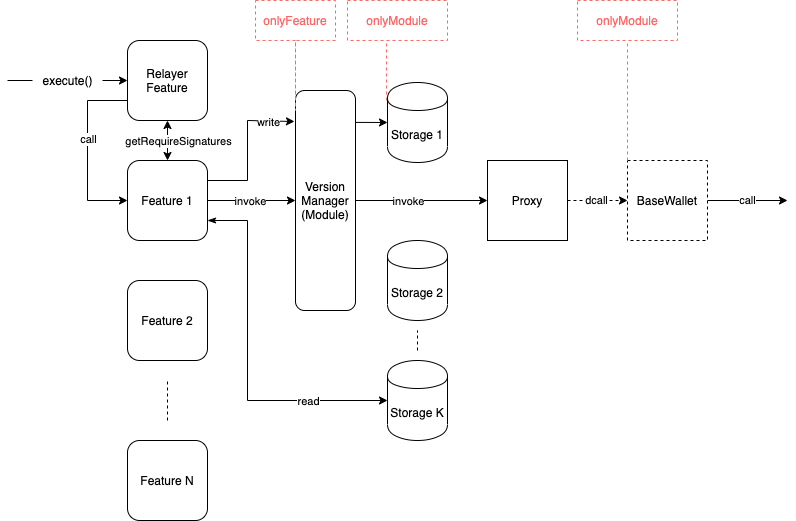
\includegraphics[width=\textwidth]{SC_Flow_2_x_final_}
    \caption{Call flow in Argent}
\end{figure}

A second group of contracts implements the functionalities of the wallet:
\begin{itemize}
    \item \textbf{Version Manager:} The Version Manager is the only module authorised for a wallet. A module is a contract that has the permission to call certain methods of a wallet on which the module is authorised. This follows a wallet design pattern introduced by Nick Johnson\footnote{https://gist.github.com/Arachnid/a619d31f6d32757a4328a428286da186 and https://gist.github.com/Arachnid/6a5c8ff96869fbdf0736a3a7be91b84e}: instead of directly calling a method in their wallet to perform a given operation, users call a method in the appropriate module contract (e.g. \emph{upgradeWallet()} in the \emph{VersionManager} module), which  verifies that the user holds the required authorization (e.g. checking that the caller is the wallet owner) and if so, calls an appropriate method on the wallet (e.g. \emph{enableStaticCall()}). 
    In a previous architecture of the Argent wallet, all functionalities were implemented as modules. Because this led to large gas cost during wallet creation and upgrades, most functionalities are now implemented as \emph{Features} (see below), which can be seen as "layer 2 modules" as they don't call the wallet directly but call it via the \emph{VersionManager} instead (see Figure~\ref{fig:sc-flow}). 
    The \emph{VersionManager} module holds a mapping of version numbers to feature bundles as well as a mapping of wallet addresses to version numbers. This allows upgrading a wallet (i.e. changing the list of features it uses) by only changing its associated version number in the \emph{VersionManager}.
    \item \textbf{Features:} As mentionned above, different functionalities of the wallet are encapsulated in different \emph{Features}. In general, a single feature contract (e.g. \emph{GuardianManager}) is used by all wallets to handle a specific set of operations (e.g. adding and revoking guardians). Features are added in bundles by the Argent multisig and each bundle is given a unique version number. A wallet can then be upgraded by its owner to use a certain bundle of features (i.e. version number).
    Features can either be called directly by the appropriate account when only one signature (e.g. owner or guardian) is required or can be called indirectly via the \emph{RelayerManager} feature (see section \ref{RelayerManager}).
    \item \textbf{Storages:} Some features store part of their states in a dedicated storage contract (see Section~\ref{sec:storage}).
    \item \textbf{Proxy Wallet:} Lightweight proxy contract that delegates all calls to a Base Wallet library-like contract. There is one proxy deployed per wallet. Note that the rationale for using the Proxy-Implementation design pattern\footnote{ introduced by Nick Johnson in https://gist.github.com/Arachnid/4ca9da48d51e23e5cfe0f0e14dd6318f} is \emph{not} to enable wallet upgradability (we use upgradable modules/features for that) but simply to reduce the deployment cost of each new wallet.
    \item \textbf{Base Wallet:} The Base Wallet is a simple library-like contract implementing basic wallet functionalities used by proxy wallets (via delegatecalls), that are not expected to ever change. These functionalities include changing the owner of the wallet, (de)authorizating modules and performing (value-carrying) internal transactions to third-party contracts.
\end{itemize}


%%%%%%%%%%%%%%%%%%%%%%%%%%%%%%%%%%%%%%%%%%%%%%%%%%%%%%%%%%%%%%%%%%%%%%%%%%%%%%%%%%%%%%%%%%%%%%%%%%%
\subsection{Upgradability}
\label{sec:upgradability}
An Argent wallet can be upgraded on two levels. In both cases, a wallet cannot be upgraded while it is locked.
\begin{itemize}
    \item \textbf{Feature Upgrade (occasional)}:
The Argent multisig can add a new version (i.e. bundle of features) to the \emph{VersionManager}. Wallet owners can then choose to upgrade their wallets to that new version by calling the \emph{upgradeWallet()} method of the \emph{VersionManager}.
    \item \textbf{Module Upgrade (rare)}:
In the rare case where the \emph{VersionManager} itself needs to be upgraded, the \emph{addModule()} method of the \emph{VersionManager} can be called to add a temporary Upgrader module that defines a migration path for a wallet. This upgrader module would remove (deauthorise) the old \emph{VersionManager} and add (authorise) the new \emph{VersionManager}. The temporary Upgrader module as well as the new \emph{VersionManager} need to be registered in the \emph{ModuleRegistry}. 
\end{itemize}

%%%%%%%%%%%%%%%%%%%%%%%%%%%%%%%%%%%%%%%%%%%%%%%%%%%%%%%%%%%%%%%%%%%%%%%%%%%%%%%%%%%%%%%%%%%%%%%%%%%
\subsection{Storage}
\label{sec:storage}
In general, each feature stores the entire state pertaining to all the wallets that use that feature. For example, the \emph{MakerV2Manager} feature stores a mapping of the vaults it manages for the wallets. Some features such as the \emph{TransferManager} make use of an additional storage contract (e.g. \emph{TransferStorage}). This is the case when their storage needs to be accessed by other features and/or to simplify the upgradability of that feature in the future.

Storage contracts include:
\begin{itemize}
\item \textbf{Lock Storage:} Used to store a wallet's lock status.
\item \textbf{Guardian Storage:} Used to store a wallet's guardians\footnote{Note that \emph{GuardianStorage} used to also be used to store a wallet's lock status, but this is now handled by \emph{LockStorage}.}.
\item \textbf{Limit Storage:} Used to store a wallet's current daily limit (and future daily limit, if it is about to change) as well as the wallet's current daily spend.
\item \textbf{Transfer Storage:} Used to store addresses that have been whitelisted by a wallet.
\end{itemize}

%%%%%%%%%%%%%%%%%%%%%%%%%%%%%%%%%%%%%%%%%%%%%%%%%%%%%%%%%%%%%%%%%%%%%%%%%%%%%%%%%%%%%%%%%%%%%%%%%%%
\subsection{Meta-Transactions}
\label{sec:meta-transactions}
Meta-Transactions are implemented via a dedicated \emph{RelayerManager} feature. It implements a permissionless method \emph{execute()} that is meant to be called by a relayer account. The relayer must pass to the \emph{execute()} function an intention and the signature(s) of this intention by the originator(s) of that intention. As described in Section~\ref{sec:eth-less-account}, this pattern allows ether-less accounts to perform operations on the wallet without the need to directly call the corresponding feature methods to do so.

The \emph{RelayerManager} calls the target feature (e.g. \emph{TransferManager} for token transfers) to determine the number of required signature(s) and to run the desired business logic (e.g. transfer of tokens).

%%%%%%%%%%%%%%%%%%%%%%%%%%%%%%%%%%%%%%%%%%%%%%%%%%%%%%%%%%%%%%%%%%%%%%%%%%%%%%%%%%%%%%%%%%%%%%%%%%%
\subsection{Features}

\subsubsection{RelayerManager feature}\label{RelayerManager}

This feature is the entry point for meta-transactions. A relayer calls the \emph{execute()} method of the \emph{RelayerManager}, which validates the signatures provided, calls the required target feature to run the business logic and optionally refunds the relayer's gas cost.

\subsubsection{GuardianManager feature}

This feature is used by the wallet owner to add or revoke a guardian. The addition or revokation of a guardian is done in two steps: an addition (or revokation) step that takes 24h to complete, followed by a confirmation (or cancellation) step that needs to be done in a subsequent 12h window period.

\subsubsection{LockManager feature}

This feature is used by guardians to lock or unlock a wallet.

\subsubsection{RecoveryManager feature}

This feature is used to change the owner of a wallet to a new owner. It can be executed immediately if the owner is still in possession of the current owner account (transfer ownership), or with a delay if the owner account is lost or stolen (recovery). Both operations need to be approved by guardians.

\subsubsection{TransferManager feature}

This feature lets users perform transfers of ETH and ERC20 tokens, approve ERC20 tokens for third-party contracts, or call third-party contracts directly. Calling contracts can be coupled with a value transfer by either providing an ETH amount or approving a spender to widthraw an ERC20 amount as part of the same transaction.

All transfers of value can be done either to whitelisted addresses without any limit, or to non-whitelisted addresses within a certain daily allowance. If the daily limit is reached for a given period, the transfer is set to a pending state and will only be executed after 24h.

\subsubsection{ApprovedTransfer feature}

This feature lets users perform instant transfers of ETH and ERC20 tokens, approval of ERC20 tokens, or contract calls to non-whitelisted addresses with the signed approval of a majority of guardians. It is also used to make instant changes to the daily transfer limit.

\subsubsection{TokenExchanger feature}

This feature lets users trade ETH and ERC20 tokens using Paraswap.

\subsubsection{CompoundManager feature}

This feature lets users lend and borrow tokens with the Compound protocol. 

\subsubsection{NftTransfer feature}

This feature lets users transfer collectibles that comply to the ERC-721 interface.  

\subsubsection{MakerManagerV2 feature}

This feature lets users invest their DAI in the DSR (Dai Savings Rate) or borrow DAI with the Maker protocol. 

\end{document}